% Verifier-Anchored RL over a Frozen LLM -- TIGHT 10-MINUTE CUT.
% ~12 frames, no section dividers. Build: make audience / make presenter (or
% latexmk -pdf this file). Presenter (slide + notes) build: define \shownotes.
\documentclass[aspectratio=169]{beamer}

\usetheme{metropolis}
\metroset{block=fill}

\usepackage{amsmath,amssymb}
\usepackage{tikz}
\usetikzlibrary{arrows.meta,positioning}

% Presenter build: define \shownotes (e.g. via the Makefile presenter target) to
% put speaker notes on a second screen; default build is the clean audience deck.
\ifdefined\shownotes
  \setbeameroption{show notes on second screen=right}
\fi

\newcommand{\pitheta}{\pi_\theta}
\newcommand{\Qpsi}{Q_\psi}
\newcommand{\piMCTS}{\pi_{\mathrm{MCTS}}}
\newcommand{\QMCTS}{Q_{\mathrm{MCTS}}}
\newcommand{\verbword}[1]{\texttt{#1}}

\title{Teaching a Small Model to Deliberate}
\subtitle{Verifier-Anchored Reinforcement Learning over a Frozen LLM}
\date{2026}
\author{}

\begin{document}

\maketitle
\note{An RL talk: a small agent with an action-value function over a structured
state, trained against rewards a deterministic verifier supplies. Everything,
MCTS included, is machinery in service of learning a small, fast policy.}

\begin{frame}{Cheap models, expensive reasoning, gamed rewards}
  \begin{itemize}
    \item Small 1--7B models are fast and deployable, but lag on GSM8K and MATH
    \item Test-time search (best-of-$N$, self-consistency, MCTS) helps but is \alert{amnesiac}: nothing is distilled back, every query pays again
    \item Dense \emph{learned} reward models close the gap by opening a Goodhart attack surface
    \item Our answer: learn a small policy; the teacher is search; the reward is a non-LLM verifier
  \end{itemize}
  \note{Inference-time search patches the symptom and never learns from it, and
  learned rewards get gamed. We turn search into a teacher and anchor reward on a
  deterministic verifier, paying the search cost once at training, not forever at
  inference.}
\end{frame}

\begin{frame}{Thesis}
  \begin{enumerate}
    \item Freeze the base LLM; learn small heads $\pitheta,\ \Qpsi$ over a structured state
    \item Cast LLM deliberation on verifiable tasks as \alert{approximate $Q$-learning over an induced context MDP}
    \item Reward is verifier-anchored, not a learned critic
    \item MCTS is a sample-efficient \emph{policy-improvement operator} supplying stronger targets, \alert{not} the central algorithm
  \end{enumerate}
  \note{The whole talk in one slide. The learnable object is the agent and its
  action-value function. Search is subordinate, producing better samples and
  targets. Because the LLM is frozen, any gain is attributable to the heads and
  the search.}
\end{frame}

\begin{frame}{The induced context MDP: structured state + seven verbs}
  \begin{itemize}
    \item \textbf{State} $s$: problem, Facts, open/closed Subgoals, Hypotheses, verifier log, answer, depth
          \begin{itemize}\item load-bearing split: \textbf{Fact} (proven) vs \textbf{Hypothesis} (tentative)\end{itemize}
    \item \textbf{Actions} $A$ ($|A|{=}7$): \verbword{DECOMPOSE}, \verbword{COMPUTE\_SUBEXPR}, \verbword{FORM\_HYPOTHESIS}, \verbword{CHECK\_CASE}, \verbword{INVOKE\_VERIFIER}, \verbword{BACKTRACK}, \verbword{COMMIT\_ANSWER}
          \begin{itemize}\item only the verb is categorical; the frozen LLM instantiates content (mostly prompt templates); a state mask gates illegal verbs\end{itemize}
    \item \textbf{Transition}: frozen LLM $+$ template \emph{samples} the next state (non-enumerable)
    \item \textbf{Reward}: ground-truth terminal $+1/-1$ from the verifier, plus a small capped intermediate shaping signal
  \end{itemize}
  \note{The state schema is the Markov bet; Fact-vs-Hypothesis lets the agent hold
  tentative claims apart from proven ones. The verb stays categorical so the
  Q-head has a fixed output and search a stable branching factor. The transition
  is sampled-only, which later forces sampled chance nodes.}
\end{frame}

\begin{frame}{A concrete trace (GSM8K)}
  \small
  \textit{P: ``A store sold 7 boxes with 6 pencils each. How many pencils?''}
  \begin{enumerate}
    \item \verbword{FORM\_HYPOTHESIS}: \texttt{hyp\_1} $=$ ``the total is 42'' (tentative)
    \item \verbword{COMPUTE\_SUBEXPR} ``$7\times 6$'' $\to 42$ (derived Fact)
    \item \verbword{INVOKE\_VERIFIER} on \texttt{hyp\_1} (SymPy) $\to$ confirmed; promoted to Fact ($+0.05$, capped)
    \item \verbword{COMMIT\_ANSWER} ``42'' $\to$ terminal verifier $\to$ reward $+1$
  \end{enumerate}
  \note{State, verb-actions, sampled transitions, and verifier reward, all
  concrete. The small promotion reward is hard-capped so it cannot be farmed above
  the terminal. At inference $B{=}0$ walks this greedily; $B{>}0$ runs MCTS.}
\end{frame}

\begin{frame}{Architecture: frozen LLM, tiny heads, offline by design}
  \begin{itemize}
    \item One frozen LLM is \emph{both} encoder and stochastic generator (one forward); embedding $=$ hidden state at \verbword{[STATE\_END]}
    \item Trainable: a small adapter $+$ multi-head $\Qpsi(s,a)$ over the 7 verbs $+$ a policy-prior head $\pitheta$ --- \alert{under 5M params}
    \item Approximate $Q$-learning: replay buffer, target net, prioritized by TD error
    \item $Q$-learning is \alert{off-policy} $\Rightarrow$ learns from \emph{any} trajectories: its own, other models', logs, human demos
  \end{itemize}
  \note{A single forward gives both the embedding and the verb-instantiator
  continuation. We train only adapter and heads, so representation drift is
  bounded and gains are attributable to the heads and search. Off-policy is the
  quiet superpower: data source and learner are decoupled.}
\end{frame}

\begin{frame}{MCTS as a policy-improvement operator, and the loop}
  \begin{columns}[T]
    \begin{column}{0.56\textwidth}
      \footnotesize
      PUCT (learned policy as prior, $\Qpsi$ as leaf value):
      \[ \arg\max_a\ \widehat{Q}(s,a) + c_{\mathrm{puct}}\,\pitheta(a\mid s)\frac{\sqrt{N(s)}}{1+N(s,a)} \]
      Chance-node mean is an honest Bellman estimator:
      \[ \tfrac{W(s,a)}{N(s,a)} \approx \textstyle\sum_{s'} P(s'\mid s,a)[R+\gamma V(s')] \]
      Distill targets: $\piMCTS$ (visits), $\QMCTS$ (chance-$Q$);
      \[ \mathcal{L}_{\mathrm{total}} = (\Qpsi-\QMCTS)^2 + \lambda\,\mathcal{L}_\pi \]
    \end{column}
    \begin{column}{0.44\textwidth}
      \centering
      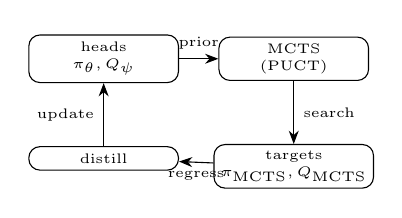
\begin{tikzpicture}[node distance=8mm and 5mm, >=Stealth, font=\tiny,
          box/.style={draw, rounded corners, align=center, inner sep=2.5pt, minimum width=19mm}]
        \node[box] (pol) {heads\\$\pitheta,\Qpsi$};
        \node[box, right=of pol] (search) {MCTS\\(PUCT)};
        \node[box, below=of search] (tgt) {targets\\$\piMCTS,\QMCTS$};
        \node[box, below=of pol] (dist) {distill};
        \draw[->] (pol) -- node[above]{prior} (search);
        \draw[->] (search) -- node[right]{search} (tgt);
        \draw[->] (tgt) -- node[below]{regress} (dist);
        \draw[->] (dist) -- node[left]{update} (pol);
      \end{tikzpicture}\\[2pt]
      \scriptsize System 1 heads, System 2 search; training shifts competence into System 1.
    \end{column}
  \end{columns}
  \note{MCTS replaces the intractable Bellman sum with sampled rollouts at a query
  state, the sampled chance node being the only available estimator. The same
  Q-learning update runs; only the targets get better because they average over
  search-guided trajectories. AlphaZero's structure inverted: the agent and Q are
  the center, search is subordinate.}
\end{frame}

\begin{frame}{Reward hacking: a verifier is necessary, not sufficient}
  \begin{itemize}
    \item Goodhart: optimize a mis-specified reward, get behavior that scores well and reasons badly
    \item A non-LLM verifier removes the \emph{learned}-reward attack surface, but a poorly specified verifier reward is still gameable
    \item We red-teamed our own intermediate shaping reward and found a farm: verifying content-free or self-authored claims for free reward
  \end{itemize}
  \begin{alertblock}{Fix by construction, not by patch}
    Tie the rewarded check to the target claim; reward only the \emph{first} success per target;
    hard-cap cumulative intermediate reward at $\tfrac{1}{5}$ of the terminal $\Rightarrow$ the ground-truth
    terminal verifier always dominates, so farming is \emph{bounded}, not just discouraged.
  \end{alertblock}
  \note{A verifiable reward is necessary but not sufficient: a badly specified
  shaping term is still hackable. We caught exactly this via adversarial review.
  The fix is structural, capping the cumulative shaping below the terminal so no
  farm can rival actually solving. Red-teaming the reward is part of the method.}
\end{frame}

\begin{frame}{Inference and deployment: one compute knob, always-on learning}
  \begin{columns}[T]
    \begin{column}{0.5\textwidth}
      \begin{block}{$B=0$ (fast)} masked $\arg\max$ over $\Qpsi$; one forward/decision; constant latency \end{block}
    \end{column}
    \begin{column}{0.5\textwidth}
      \begin{block}{$B>0$ (search)} PUCT MCTS for $B$ sims; sample the visit-count policy \end{block}
    \end{column}
  \end{columns}
  \begin{itemize}
    \item Same trained heads; one dial traces a compute-vs-accuracy frontier, no retraining
    \item Off-policy $+$ verifier-anchored $\Rightarrow$ keep learning in deployment from any verifier-style signal, incl. \alert{user thumbs up/down}
    \item Per-user adapters absorb idiosyncratic feedback; the verifier stays the anchor that bounds drift
  \end{itemize}
  \note{Two modes, one learned actor with different search on top; $B$ becomes a
  user-controlled dial. Because the heads were distilled from MCTS targets, fast
  mode already carries much of the benefit. Deployment traffic is just more
  off-policy experience, so the model can keep improving, anchored by the verifier.}
\end{frame}

\begin{frame}{Positioning and defensible novelty}
  \begin{itemize}
    \item \textbf{AlphaZero / expert iteration}: we \alert{invert} it --- agent and $\Qpsi$ central, search optional
    \item \textbf{Verifier-anchored reasoning} (PRMs, AlphaProof, DeepSeek-R1): verifier-vs-aesthetic asymmetry is load-bearing; \verbword{INVOKE\_VERIFIER} is a callable verb
    \item \textbf{VerifierQ}: verifier-as-\emph{action} not verifier-as-$Q$; online distilled targets; categorical multi-head $Q$
    \item \textbf{vs STaR / ReST-EM / Math-Shepherd}: per-step $\QMCTS$ as a genuine Bellman target, not trajectory-level or a process-reward model
  \end{itemize}
  \note{We inherit AlphaZero's joint search-and-learning but invert its center, so
  non-search baselines are first-class. The afterstate split is borrowed, not
  claimed novel; novelty is its application to the non-enumerable LLM-induced
  transition.}
\end{frame}

\begin{frame}{How we will evaluate (the plan, not results)}
  \begin{itemize}
    \item GSM8K and MATH; baseline grid fixed in advance: base-greedy, best-of-$N$, self-consistency, STaR/ReST-EM, AlphaZero-for-reasoning, PRM-guided
    \item \alert{Pre-registered} hypotheses and the headline frontier figure committed \emph{before} training; $\geq 3$ seeds, $\geq 8$ replicates, mean $\pm$ std
    \item Holm--Bonferroni across the FLOP $\times$ benchmark grid; explicit compute-leak threat model
  \end{itemize}
  \begin{block}{Honest frontier accounting}
    $x$: total inference FLOPs (charge \emph{every} forward inside the $B$ simulations, not just the root); $y$: accuracy; FLOP-matched curves. Pilot: generation dominates prefill $\approx 79{:}1$ per decision.
  \end{block}
  \note{Methodology, not a victory lap; we deliberately do not lean on current
  pilot numbers, and strong results are in progress. Honest FLOP accounting is
  what makes beating best-of-N mean we learned something, not that we spent more
  compute.}
\end{frame}

\begin{frame}[standout]{Vision}
  A small, fast model that \emph{learns to deliberate} over structured states,\\
  anchored by verifiable (non-learned) rewards.\\[0.8em]
  Offline today, online-continual in deployment, one test-time compute knob.\\[0.8em]
  \footnotesize MCTS earns its keep only as the operator that manufactures stronger targets.
  \note{The takeaway is the RL-first frame: learn a small policy and Q over a
  structured state with verifiable rewards; search teaches the heads. Fast by
  default, thinks harder on demand, keeps learning after deployment. Next: the
  pre-registered frontier at scale.}
\end{frame}

\end{document}
